\documentclass[12pt,letterpaper]{article}
\usepackage[utf8]{inputenc}
\usepackage[spanish]{babel}
\usepackage{graphicx}
\usepackage[left=2cm,right=2cm,top=2cm,bottom=2cm]{geometry}
\usepackage{graphicx} % figuras
% \usepackage{subfigure} % subfiguras
\usepackage{float} % para usar [H]
\usepackage{amsmath}
%\usepackage{txfonts}
\usepackage{stackrel} 
\usepackage{multirow}
\usepackage{enumerate} % enumerados
\renewcommand{\labelitemi}{$-$}
\renewcommand{\labelitemii}{$\cdot$}
% \author{}
% \title{Caratula}
\begin{document}

% Fancy Header and Footer
% \usepackage{fancyhdr}
% \pagestyle{fancy}
% \cfoot{}
% \rfoot{\thepage}
%

% \usepackage[hidelinks]{hyperref} % CREA HYPERVINCULOS EN INDICE

% \author{}
\title{Caratula}

\begin{titlepage}
\begin{center}
\large{UNIVERSIDAD PRIVADA DE TACNA}\\
\vspace*{-0.025in}
\begin{figure}[htb]
\begin{center}

\includegraphics[width=8cm]{./Imagenes/logo}
\end{center}
\end{figure}
\vspace*{0.15in}
INGENIERIA DE SISTEMAS  \\

\vspace*{0.5in}
\begin{large}
TITULO:\\
\end{large}

\vspace*{0.1in}
\begin{Large}
\textbf{Informe Laboratorio N° 01 } \\
\end{Large}

\vspace*{0.3in}
\begin{Large}
\textbf{CURSO:} \\
\end{Large}

\vspace*{0.1in}
\begin{large}
INTELIGENCIA DE NEGOCIOS\\
\end{large}

\vspace*{0.3in}
\begin{Large}
\textbf{DOCENTE(ING):} \\
\end{Large}

\vspace*{0.1in}
\begin{large}
 Patrick Cuadros Quiroga\\
\end{large}

\vspace*{0.2in}
\vspace*{0.1in}
\begin{large}
Integrantes: \\
\begin{flushleft}
Perez Mamani Nilton Edy		\hfill	(2015053223) \\
\end{flushleft}
\end{large}
\end{center}

\end{titlepage}


\tableofcontents % INDICE
\thispagestyle{empty} % INDICE SIN NUMERO
\newpage
\setcounter{page}{1} % REINICIAR CONTADOR DE PAGINAS DESPUES DEL INDICE

\begin{center}
    PRACTICA DE LABORATORIO N° 01
\end{center}

\section{OBJETIVOS}
Elaboración de Dashboards en Power BI

\section{REQUERIMIENTOS}

\begin{itemize}

- Conocimientos básicos de administración de base de datos Microsoft   SQL Server.
\\- Conocimientos básicos de SQL.
\\- Microsoft SQL Server 2016 o superior
\\- Base de datos AdventureWorks2016 o superior
\\- Power BI Desktop.
\\- Tener una cuenta Microsoft registrada en el Portal de Power Bi.
\end{itemize}

\section{DESARROLLO} 

\begin{itemize}
1. Iniciar Power BI Desktop.
\end{itemize} 

\begin{center}
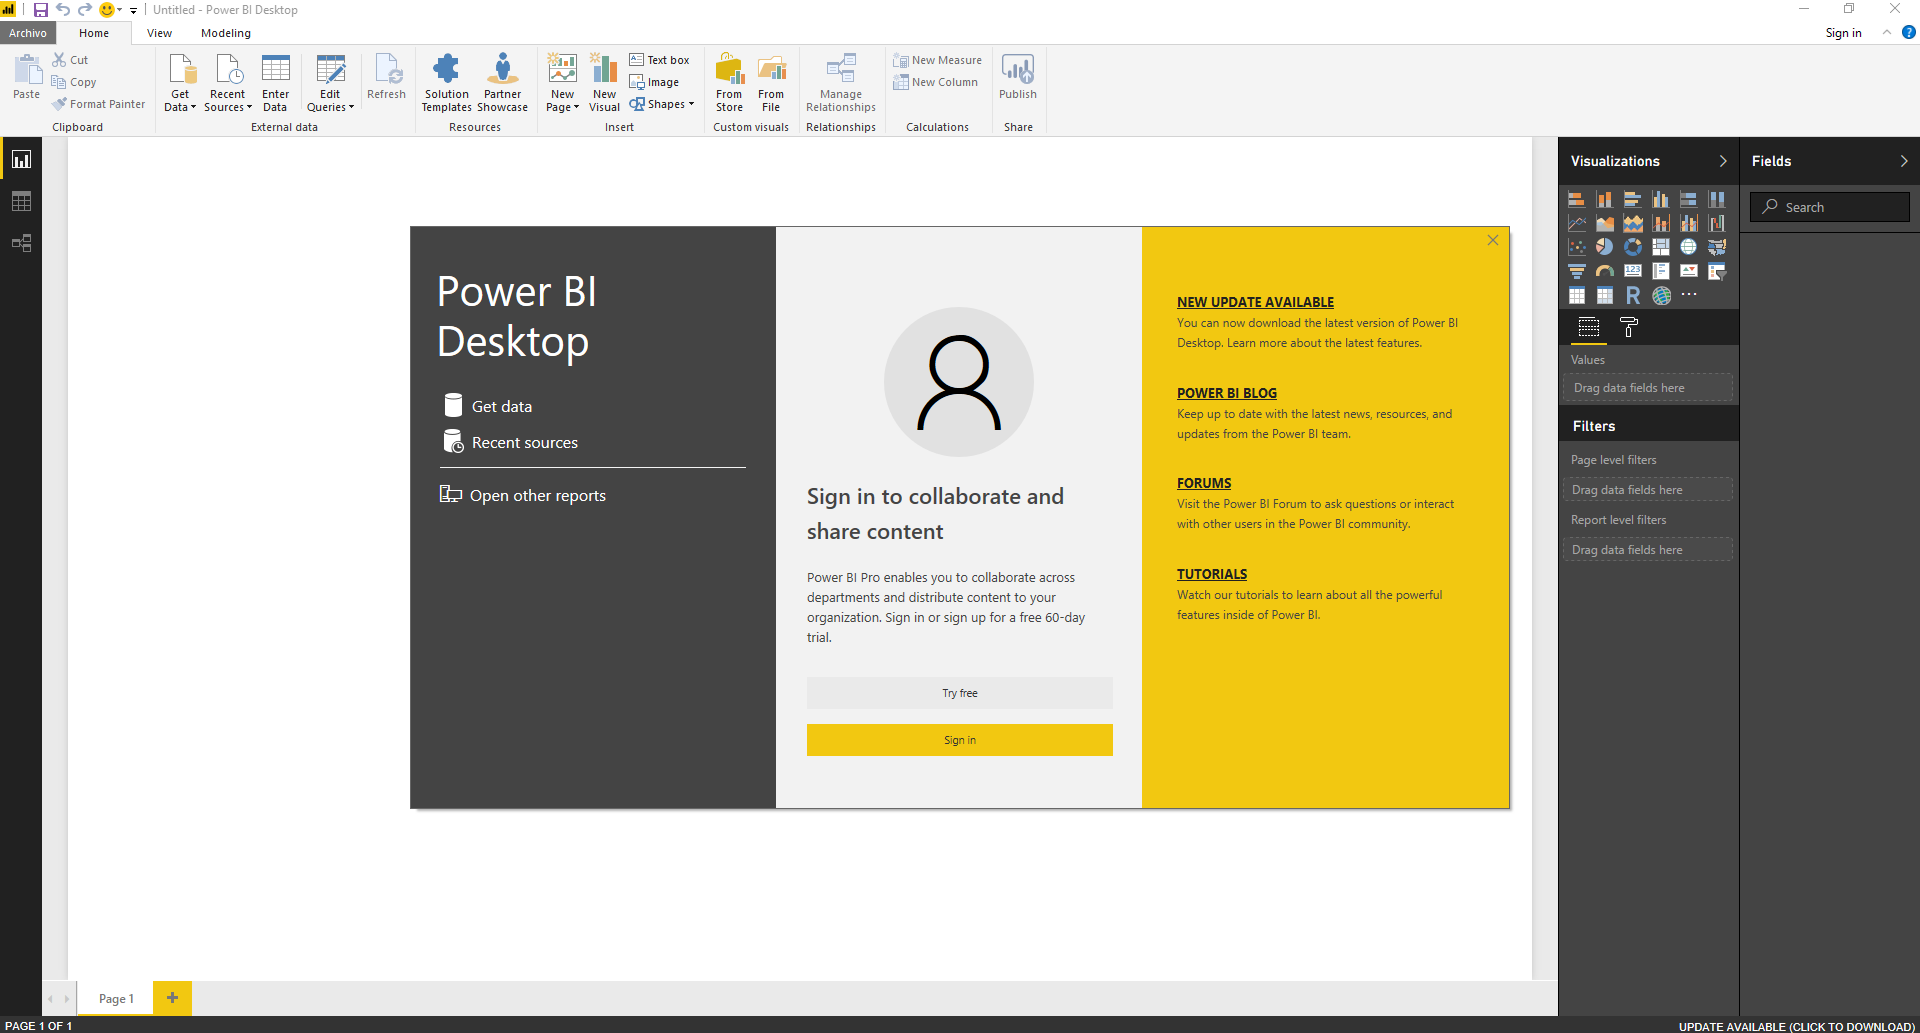
\includegraphics[width=15cm]{./Imagenes/imagen1} 
\end{center}

\begin{itemize}
2. Conectar a SQL Server desde Power BI Desktop 
\end{itemize} 

\begin{center}
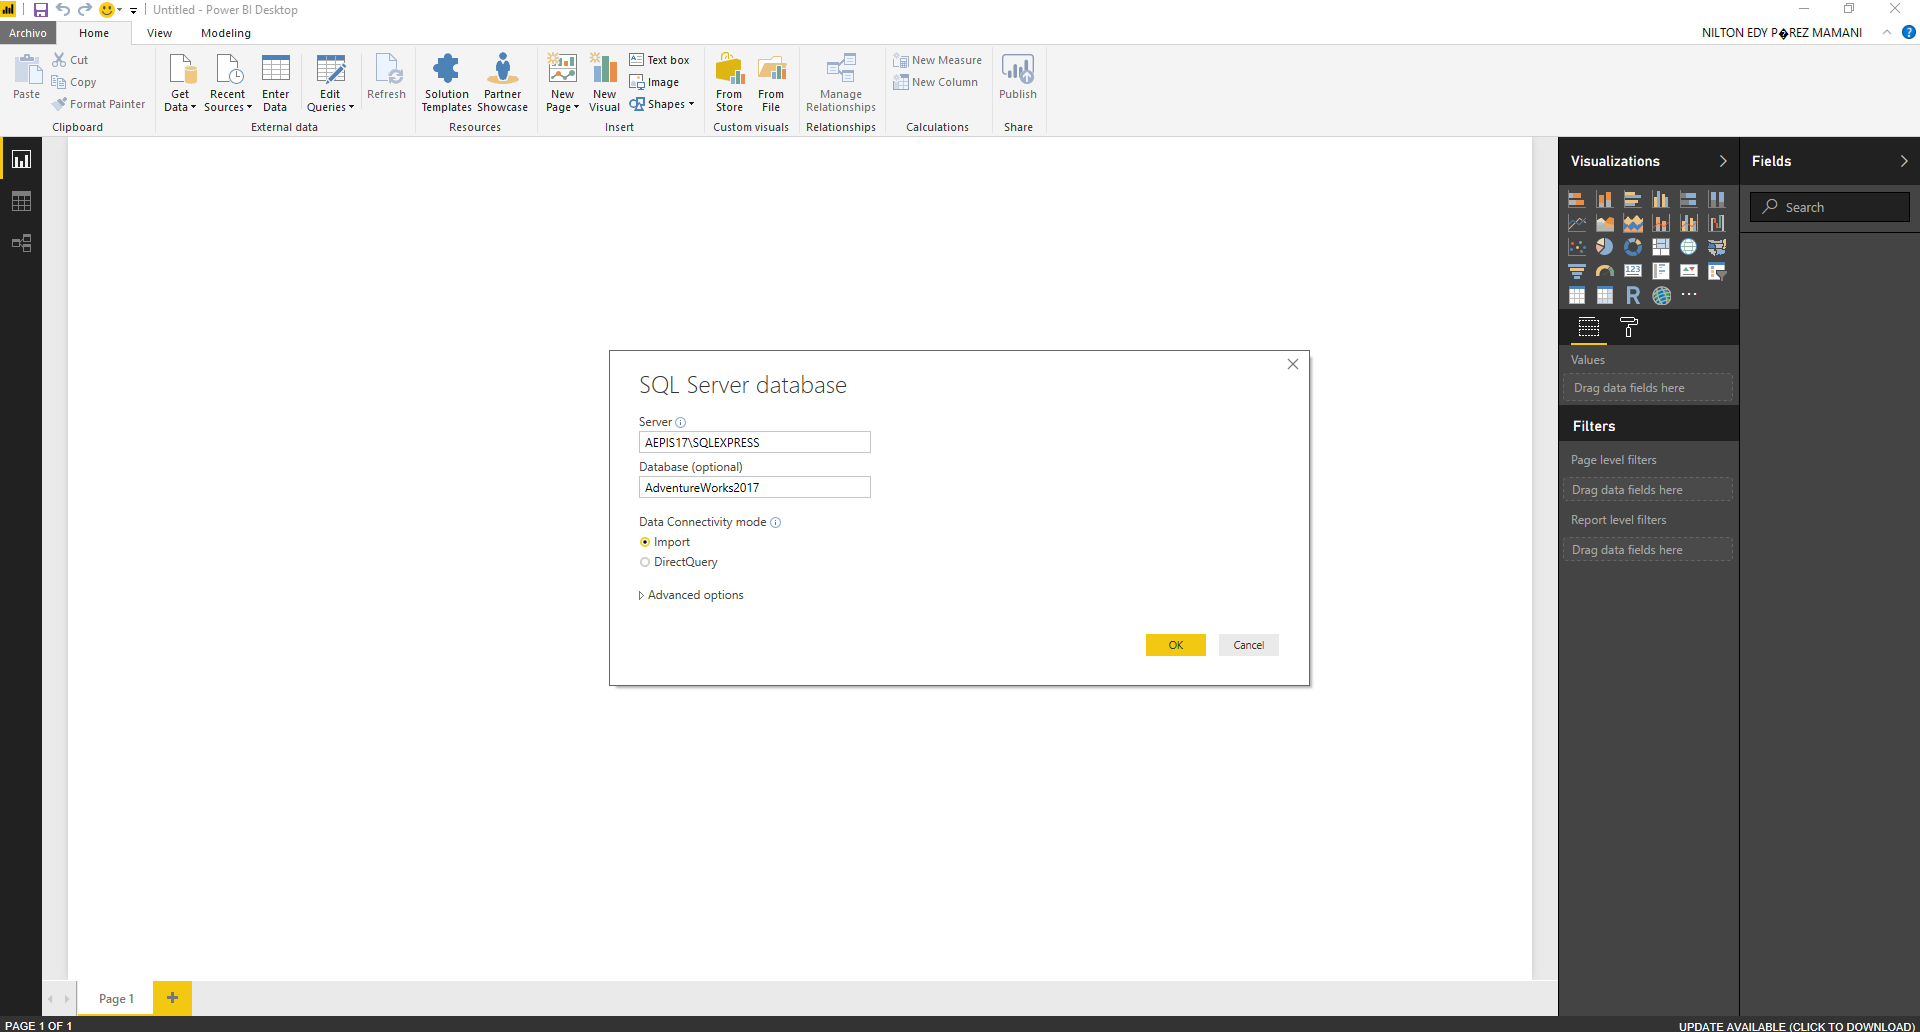
\includegraphics[width=15cm]{./Imagenes/imagen2} 
\end{center}

\begin{itemize}
3. Generar un reporte que muestre a todo el personal de ventas 
\end{itemize} 

\begin{center}
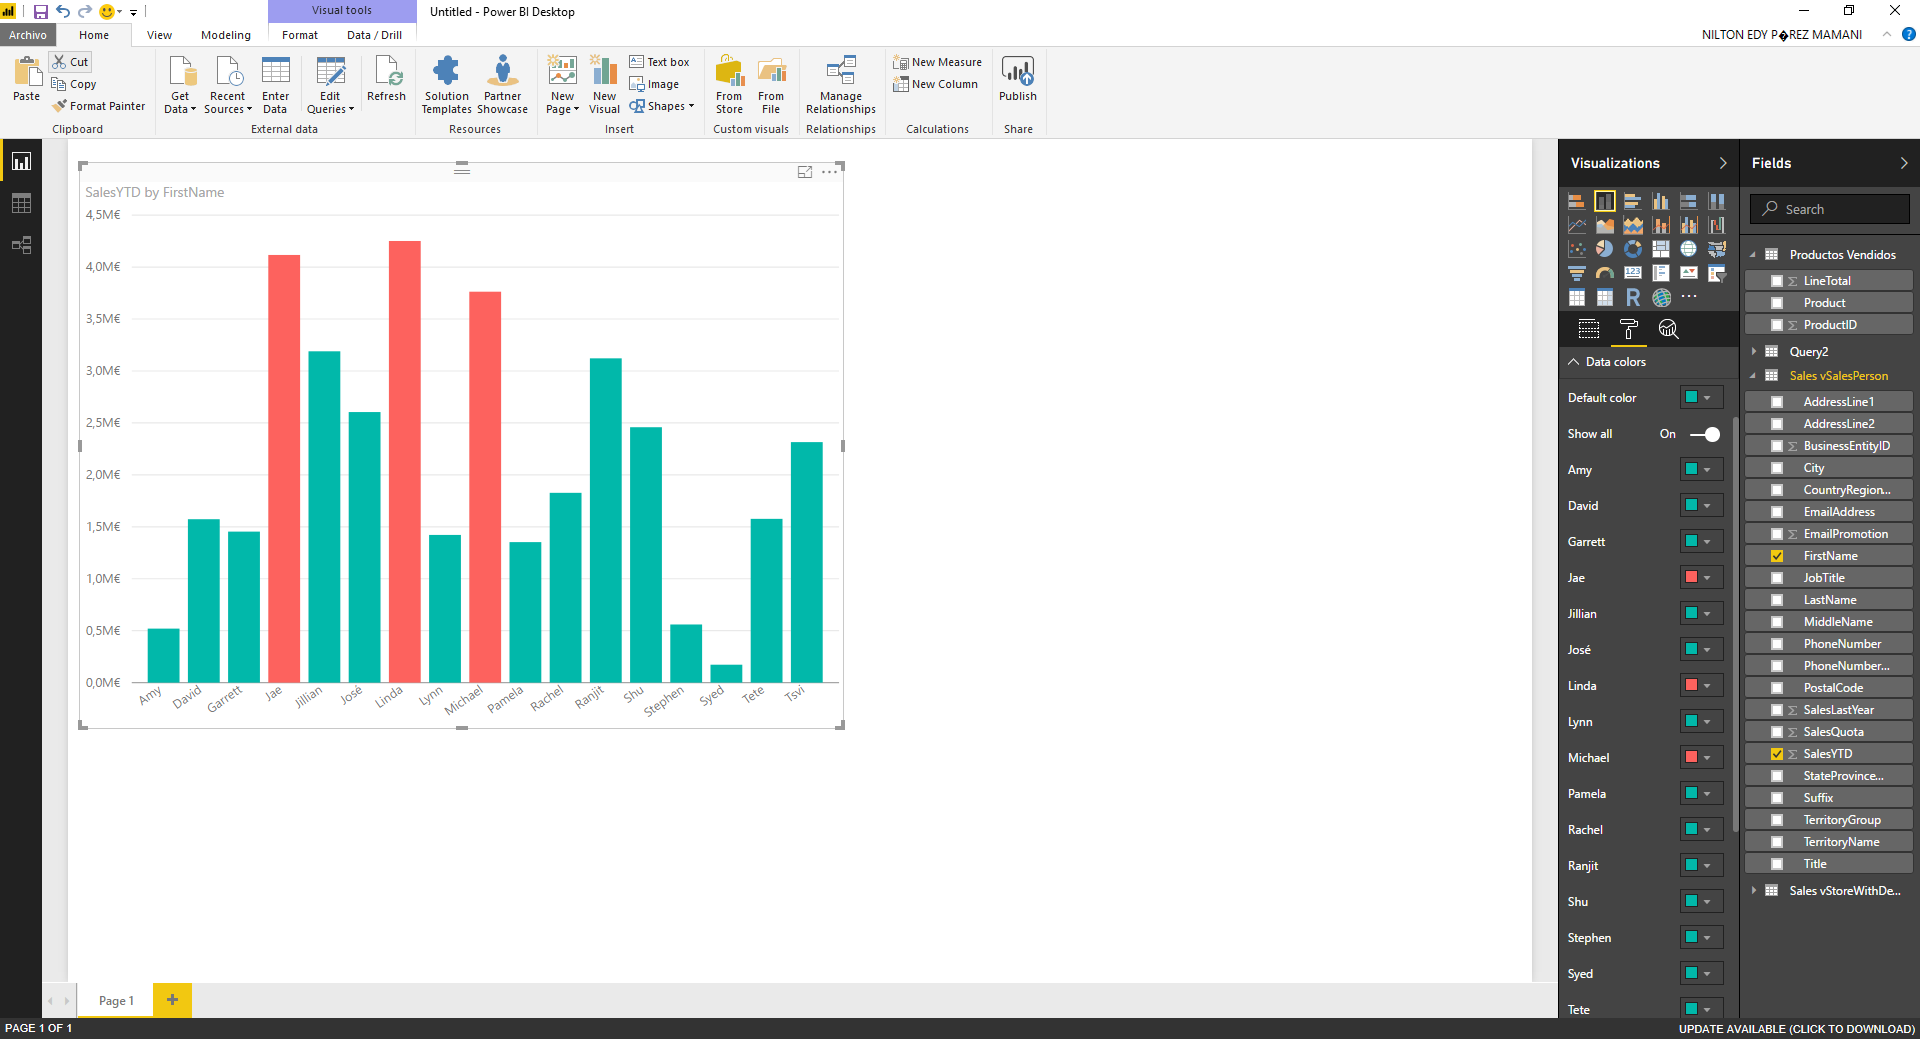
\includegraphics[width=15cm]{./Imagenes/imagen3} 
\end{center}

\begin{itemize}
4. Generar un area de reporte que muestre todo los resultados que indica el trabajo
\end{itemize} 

\begin{center}
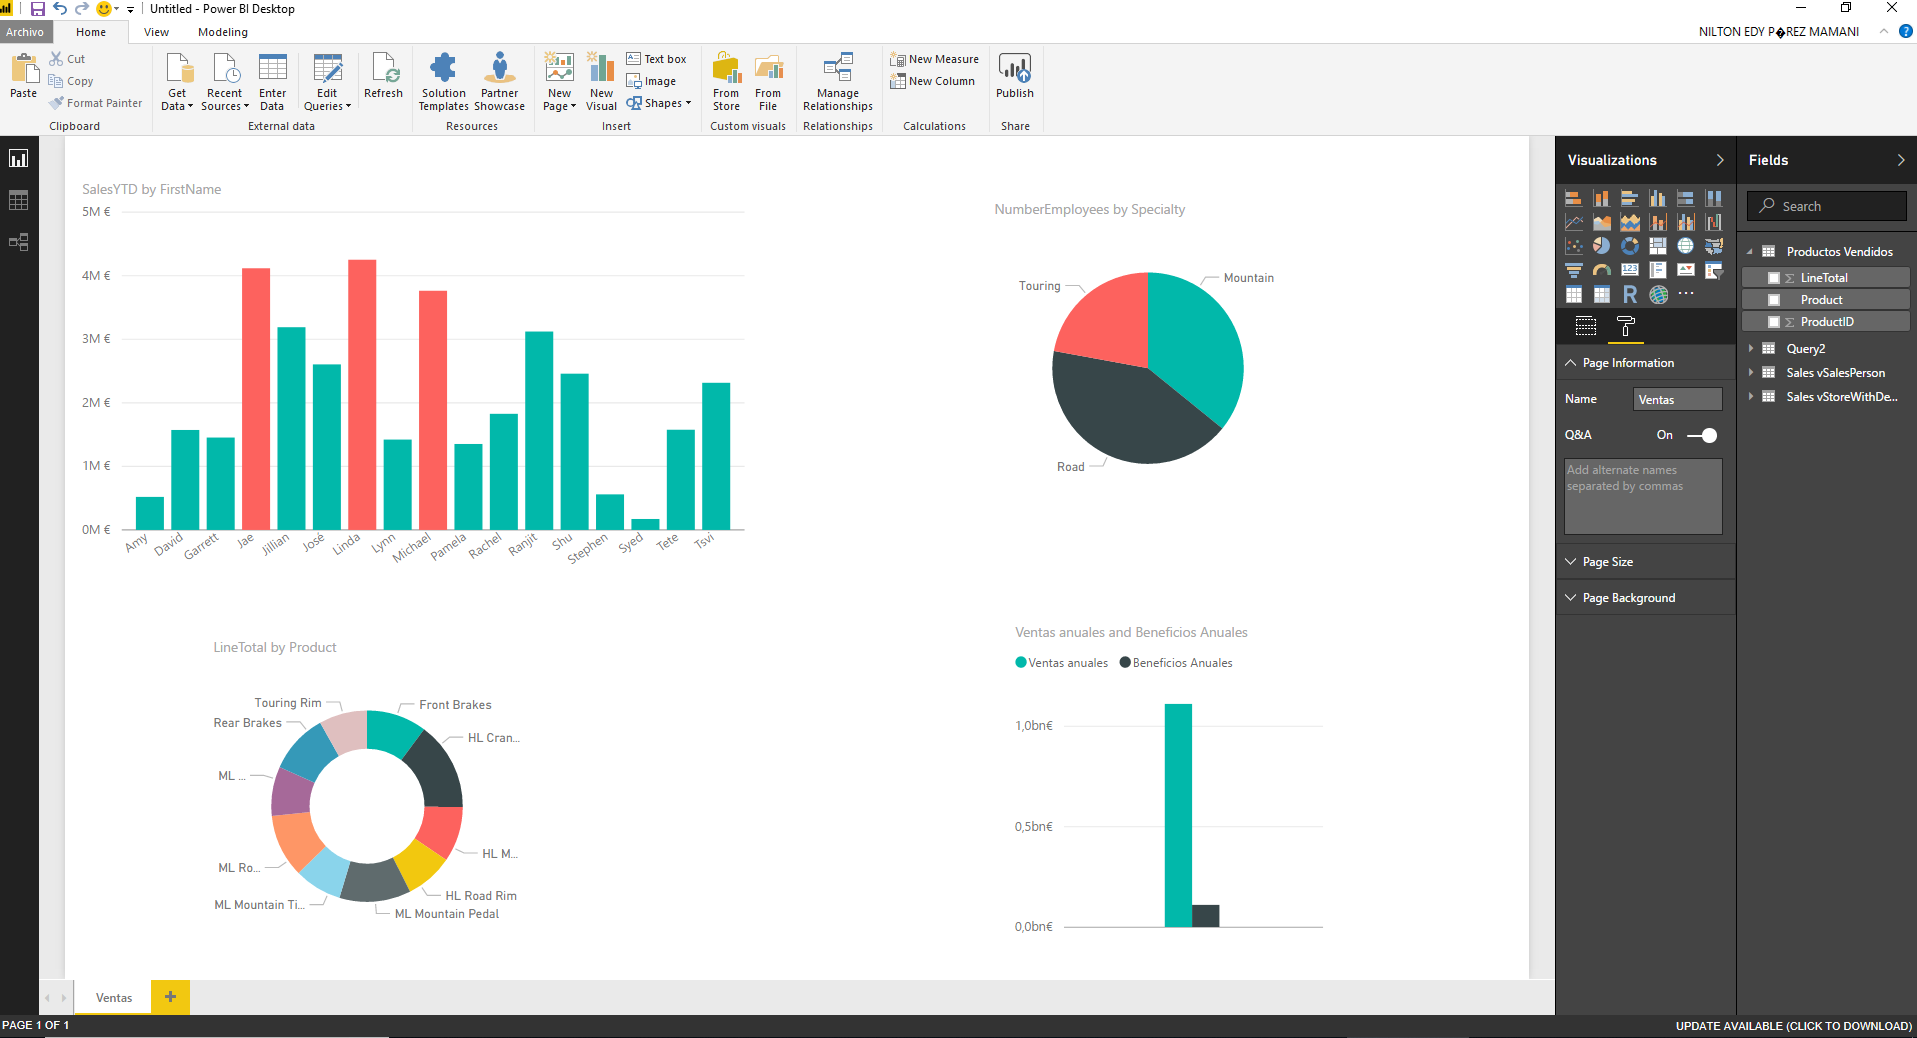
\includegraphics[width=15cm]{./Imagenes/imagen4} 
\end{center}

\begin{itemize}
5. Publicar el reporte en el portal de Power BI
\end{itemize}

\begin{center}
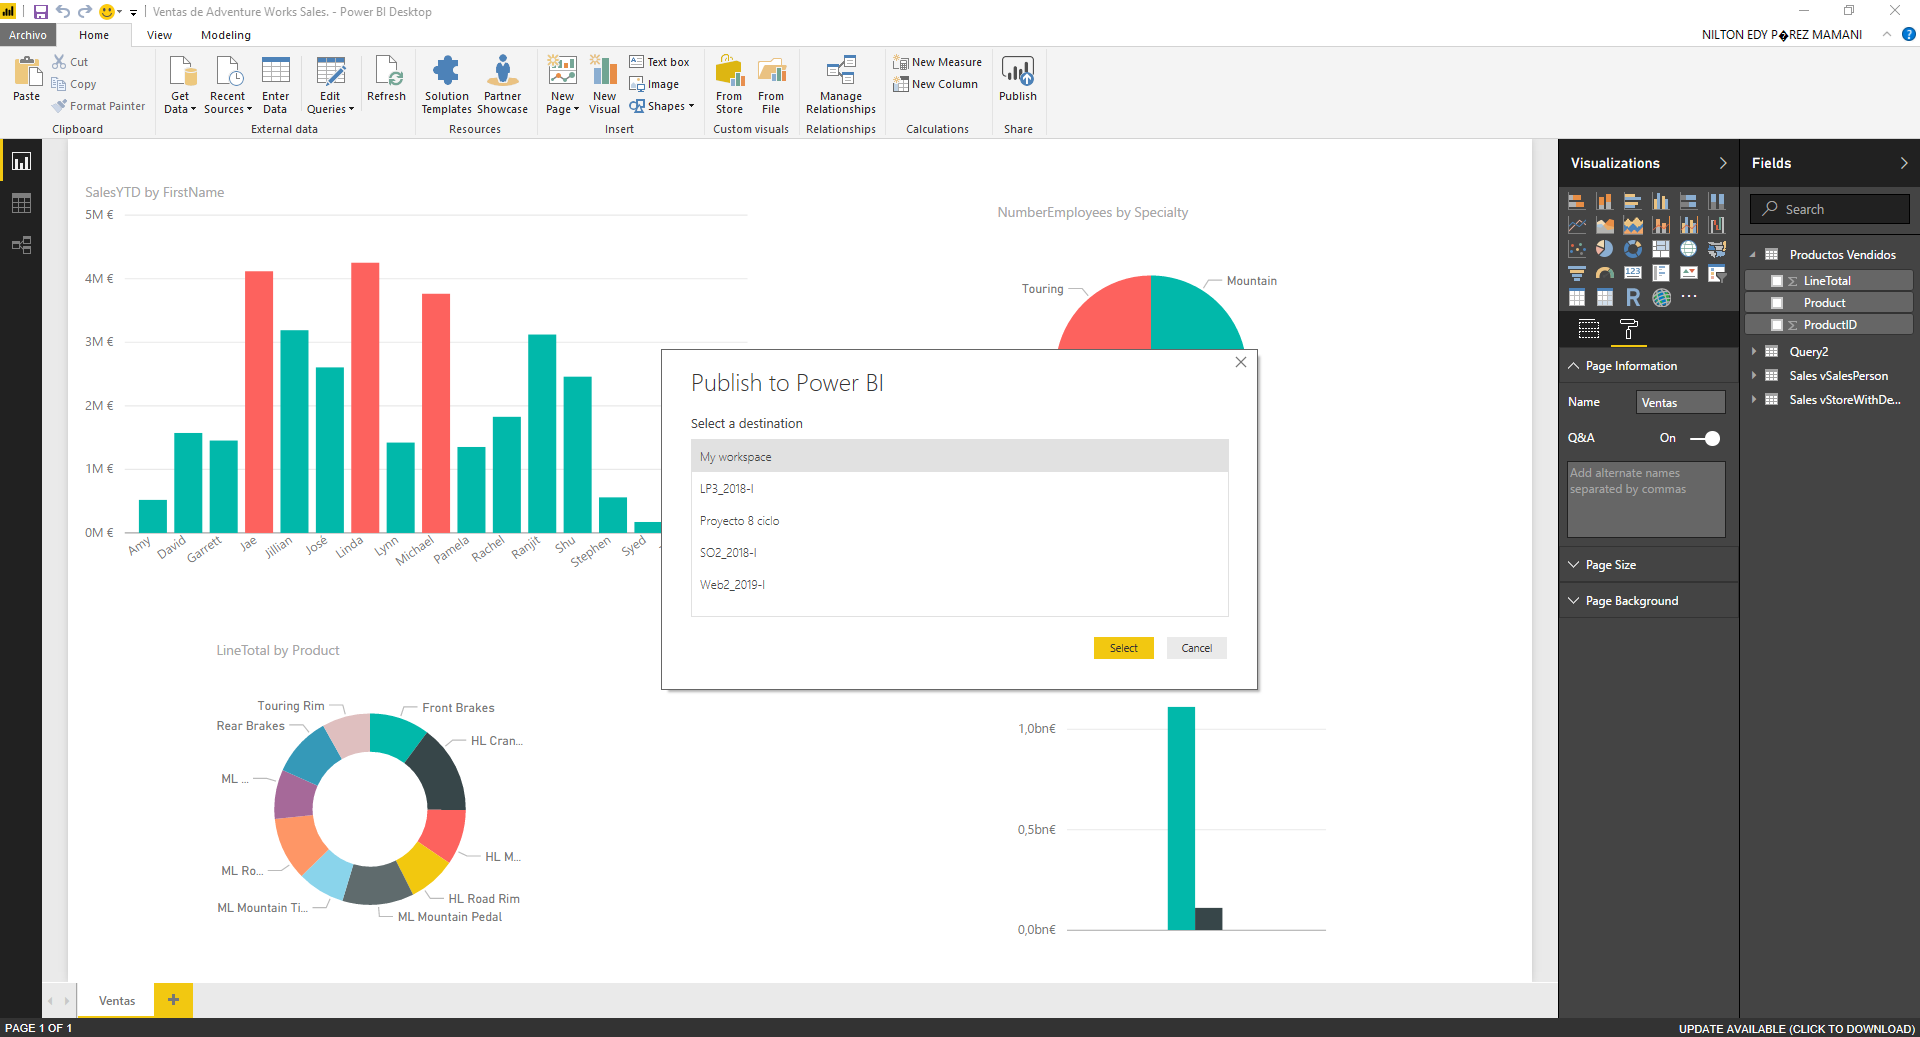
\includegraphics[width=15cm]{./Imagenes/imagen5} 
\end{center}

\begin{itemize}
6. Resultado final
\end{itemize}

\begin{center}
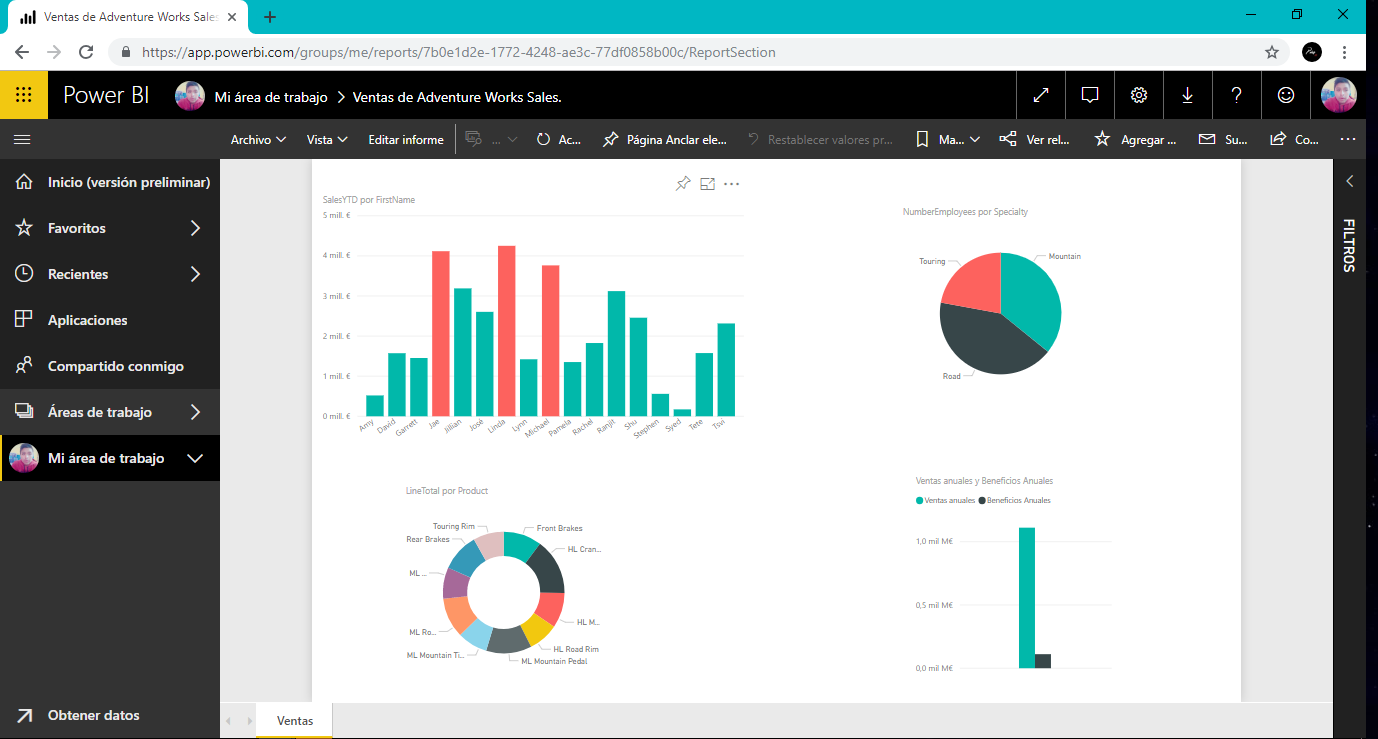
\includegraphics[width=15cm]{./Imagenes/imagen6} 
\end{center}

\end{document}
